% this is a part of the habilitation thesis of Max Neunhoeffer

\chapter{Matrices over finite fields}

This chapter covers the implementation of the basic operations for matrices 
over finite fields. We begin with a description of a new concrete 
representation of such matrices on nowadays computers in 
Section~\ref{sec:ffematrices}, both in main memory and on storage.
We then analyse the performance and complexity of matrix arithmetic 
for this new representation in Section~\ref{sec:matarith} and compare
it to previous implementations. In Section~\ref{sec:basalgmat}, we give
an overview over the most basic algorithms for finite field matrices,
before we conclude this chapter with the description of a new method
to compute minimal polynomials of matrices over finite fields in
Section~\ref{sec:charminpoly}, which is used to compute projective orders
of matrices.

%FIXME

\section{Representing vectors and matrices over finite fields}
\label{sec:ffematrices}

If you already know something about compact vectors and matrices over 
finite fields you can safely skip the next subsection and directly
proceed to Section~\ref{ssec:cvec}. We first explain the basic idea.

\subsection{The idea}

If $p$ is a prime then elements of the finite field $\F_p$ with $p$
elements can be represented by the integers $0, 1, \ldots, p-1$. Thus,
storing one such element on a computer needs only $\lceil \log_2(p)
\rceil$ bits. The finite extension field  $\F_q$ with $q = p^k$ elements 
is built
as quotient $\F_p[x]/c_k \F_p[x]$ using the Conway polynomial
$c_k$ (see \cite{Nickel} or on the web at \cite{ConwayFL}). Since the
Conway polynomials are monic by definition, an element
of\, $\F_q$ can be represented by one polynomial over\, $\F_p$ of degree 
less then $k$ and thus by storing $k$ elements of\, $\F_p$ using $\lceil
\log_2(p^k) \rceil$ bits.

Since linear algebra operations over finite fields can be performed
rather efficiently by modern microprocessors, the limiting factor 
for such computations is memory access. Therefore, it is performance
critical to store vectors and matrices using as little memory as possible,
and to choose the data structure in a way that allows for fast memory
access. We call such memory efficient data structures ``compact''.

This idea is quite old (see ADDREFERENCE) and has already been used
extensively (see for example \cite{CMeatAxe} or \cite{GAP4} or
various other systems).

There is a fundamental difference between the characteristic $p=2$ case
and all other characteristics. The reason for this is that in
characteristic $2$ the addition of vectors can be implemented by using
the XOR (exclusive or) operation available in every microprocessor
instruction set. In odd characteristic, the available instructions
do not fit so well to finite field arithmetic. Therefore, previous
implementations mostly rely on table lookups to perform arithmetic
operations. Since the memory space available for lookup tables is
limited, this method is limited to relatively small fields (usually up to
fields with $256$ elements) and has to use single byte accesses
as opposed to processor word accesses, for which modern machines
seem to be optimised. These limitations seem to become more serious
as word lengths in standard microprocessors increase.

The main novelty in the approach presented here is to overcome this
problem by choosing the data structures in a way that allows to use
processor word operations for all arithmetic operations in all
characteristics. Also this idea has been used before (see
\cite{EssenLinAlg}), however, no implementation of this seems to
be available any more and, more importantly, the approach still
insisted on storing whole elements of\, $\F_q$ in one machine word.
We will pack as many prime field elements as possible into a machine
word and distribute the various prime field coefficients of a single
element of\, $\F_q$ into distinct machine words to allow for better
memory usage in the case of extension fields.


\subsection{Compact vectors}
\label{ssec:cvec}

We first describe in detail how a vector of length $n$ over the field
$\F_q$ with $q=p^k$ elements is stored on a machine with word length $32$ 
or $64$ bits respectively. The ideas for the step from $32$ to $64$ bits
can be applied analogously for future microprocessors with even larger
word length. We ignore architectures with funny word lengths not being
a multiple of $32$ bits.

Let $e$ be $\lceil \log_2(2p-1)\rceil$ for $p > 2$ and $1$ for $p=2$. 
This is the number of bits
necessary to store an integer in the range $0,1, \ldots, 2p-2$ except
for $p=2$, where it is $1$. This number $e$ is the number of bits we 
reserve for every prime field element we want to store. For $p=2$ this
is evidently best possible, whereas for odd $p$, we seem to waste
one bit per prime field element, since we seem to need only store
numbers in the range $0,1,\ldots p-1$. This additional bit in the
data structure allows us to represent a sum of two numbers in the
range $0,1,\ldots, p-1$ using $e$ bits in odd characteristic.

We start with the prime field case $q=p$.

We pack as many prime field elements as possible into a machine
word, that is, $w := \lfloor 32/e \rfloor$ prime field elements per word
on a machine with word length $32$ bit. On machines with $64$ bits
we pack $w := 2 \lfloor 32/e \rfloor$ prime field elements into one word.
Note that we do not use $\lfloor 64/e \rfloor$ elements which can be one
more, since then the conversion between the different data formats for
different word lengths becomes too expensive and awkward.

We always imagine the least significant bit in a machine word as being 
on the right hand side. To store a vector, we start filling machine words 
from right to left, always using $e$ bits for one prime field element and
packing $w$ prime field elements into a word.

We illustrate this layout in the following example for $p=5$ and thus
$e=4$ on a machine with $32$ bit word length:

\begin{verbatim}
  bit             3322|2222|2222|1111|1111|1100|0000|0000
  number:         1098|7654|3210|9876|5432|1098|7654|3210
  prime field         |    |    |    |    |    |    |
  element number: 7777|6666|5555|4444|3333|2222|1111|0000
\end{verbatim}

Within each block of $e$ bits, we represent prime field elements
by the binary representation of a number in the range $0,1,\ldots,p-1$
with the least significant bit of this binary representation on the
right hand side. Thus, in our example $1+1+1+1 \in \F_5$ would be
represented by the bit sequence \texttt{0100} and $1+1+1$ by \texttt{0011}.
Note that the most significant bit in this representation is always $0$.

The first $w$ prime field elements in a vector are stored in the first
machine word of the vector, the next $w$ in the next word and so on.

We proceed now to the extension field case $q=p^k$. Let $e$ and $w$ be
exactly the same values as above. We now have to store $k$ prime field
elements for every element of $\F_q = \F_p[x]/c_k\F_p[x]$, namely the 
coefficients of the unique residue class representative of degree smaller 
than $k$, where $c_k$ is the Conway polynomial used to construct the 
finite field extension $\F_q$ over $\F_p$ (for details see \cite{Nickel}
or on the web \cite{ConwayFL}). Namely, if $a \in \F_q$ is represented by
the polynomial $\sum_{i=0}^{k-1} a_i x^i$, then we have to store the prime 
field elements $a_0, a_1, \ldots, a_{k-1}$. 

In a compact vector of length $n$ of elements of $\F_q$ we distribute
those numbers in the following way: The first $k$ machine words in the
memory representation of the vector are used to store the first $w$
elements of the vector. The first machine word holds all the coefficients
$a_0$ of those $\F_q$ elements, the second the coefficients $a_1$ and so
on. Since one machine word can hold up to $w$ prime field elements this
fills the first $k$ words rather satisfactorily. The second $k$ machine words
in the vector then hold the vector elements with indices 
$w+1, w+2, \ldots, 2w$ in exactly the same way.

Note again that for machines with a word length of $64$ bit we choose the
value $w$ only twice as big as for $32$ bit machines even if one more
prime field element would fit into the machine word.

The only natural limit of this implementation is that 
$\lceil \log_2(2p-1) \rceil$ must be smaller or equal to the word length
of the microprocessor.

We can now explain, how we can add vectors in the above representation
only by doing a series of word operations.

\subsection{Adding compact vectors}

The basic addition formula for finite field elements is rather simple:
For prime field elements we just have to add two numbers in the range 
from $0$ to $p-1$, and
subtract $p$, if the sum is greater or equal to $p$. The extension
field elements are done component-wise. However, we have to solve
the problem of doing this simple operation using word operations and 
thus doing this for $w$ prime field elements at the same time.
This is easy for $p=2$, since we can use the standard XOR (exclusive or)
operation.

The idea to overcome this problem for $p > 2$ is the following. 
Assume $a$ and $b$
are two integers in the range from $0$ to $p-1$. By adding
$2^{e-1}-p$ to the sum $a+b$ we get $t := a+b+2^{e-1}-p$, which
has the property, that $t \ge 2^{e-1}$ if and only if $a+b \ge p$
(remember $2p-1 \le 2^e$ and thus $p-1 < 2^{e-1}$). That is, if
the number $t$ is represented using binary expansion with $e$ bits,
then the most significant bit is set if and only if $a+b \ge p$.

This idea is now used for two words $a$ and $b$, containing $w$
prime field elements each. Every prime field element uses exactly $e$ bits
in its word and we call these sections of $e$ adjacent bits in a word 
``components'' for the moment. 

We prepare an ``offset'' word $o$ that contains in each component the
number $2^{e-1}-p$ and a ``mask'' word $m$ that contains in each component
the number $2^{e-1}$ meaning, that in each component only the most significant
bit is set and all others are zero. In addition, we keep a word $n$
containing the number $p$ in each component.

The finite field sum $c$ of $a$ and $b$ is now computed in the following way:
First $s := a+b$ and $t := a+b+o$ are computed. We then use an AND 
operation for words to extract exactly the most significant bits of
those components, in which the sum was greater or equal to $p$.
This is done by computing $r := t \ \&\  m$ (we use the \& symbol to
indicate bit-wise AND operations). Bit-shifting
the word $r$ by $e-1$ bits to the right (we use the notation
$r \gg (e-1)$ for this) and subtracting the
result from $r$ now results in a word $u := r - (r \gg (e-1))$
having the number $2^{e-1}-1$
in those components, in which the sum was greater or equal to $p$ and
$0$ in the others. Finally, doing a bitwise AND operation of $u$ with
$n$ results in exactly the right word to subtract from $s$ to get
the correct result.

Thus, the complete formula is
\[ a+b - \Big(\big(r - (r \gg (e-1))\big) \ \&\ n \Big)
   \qquad \mbox{where}\quad r = (a+b+o) \ \&\  m \]

We illustrate this by an example for $p=3$ on a machine with
$32$ bit word length. In this case, $e = 3$ and $w = 10$. We want to
add the words shown below in the rows depicted by \texttt{a} and \texttt{b}.
We also show the prepared words $o$, $m$, and $n$. The bits marked
with \texttt{X} are not used and are all equal to zero.

\begin{verbatim}
  bit             33|222|222|222|211|111|111|110|000|000|000
  number:         10|987|654|321|098|765|432|109|876|543|210
                    |   |   |   |   |   |   |   |   |   |
  a:              XX|000|010|001|000|010|001|000|010|001|000
  b:              XX|000|010|010|010|001|001|001|000|000|000
  o:              XX|001|001|001|001|001|001|001|001|001|001
  m:              XX|100|100|100|100|100|100|100|100|100|100
  n:              XX|011|011|011|011|011|011|011|011|011|011
\end{verbatim}

In the following table we show some intermediate results and repeat
the input values for easier verification:

\begin{verbatim}
  a+b:            XX|000|100|011|010|011|010|001|010|001|000
  a+b+o:          XX|000|101|100|011|100|011|010|011|010|001
  r:              XX|000|100|100|000|100|000|000|000|000|000
  u:              XX|000|011|011|000|011|000|000|000|000|000
  u&n:            XX|000|011|011|000|011|000|000|000|000|000
  result:         XX|000|001|000|010|000|010|001|010|001|000
  a:              XX|000|010|001|000|010|001|000|010|001|000
  b:              XX|000|010|010|010|001|001|001|000|000|000
\end{verbatim}

Of course, it is a coincidence here that $u$ is equal to 
$u \ \&\ n$, since $p = 2^{e-1}-1$.

This means, that the addition of two words containing $w$ prime field
elements can be done in $7$ word operations for $p > 2$. For the
$p=2$ case, we only need one XOR operation. Thus we have proved:

\begin{Prop}[Addition of compact vectors]
\label{addvec}
We assume a machine with $32$ bit word length. For $2 < p < 2^{31}$,
two compact vectors of length $n$ over the field of $q=p^k$
elements can be added using $7k\cdot \lceil n/w \rceil$ word operations
(plus memory fetches and stores), where $w = \lfloor 32/e \rfloor$
and $e = \lceil \log_2(2p-1) \rceil$. 

For $p=2$, only $k \cdot \lceil n/32 \rceil$ word operations are needed.

For machines with $64$ bit word length, the number of word operations
is halved in both cases and we can work with primes $p < 2^{63}$.
\end{Prop}
\Proof See above. \ProofEnd

\begin{Rem}
Note that since the amount of memory needed for a vector of length $n$
is $k \cdot \lceil n/w \rceil$ for $p > 2$ and $\lceil n/32 \rceil$ for
$p=2$ this means that the addition needs $7$ word operations for each
word of a vector for $p>2$ and $1$ word operation for $p=2$.

Assuming a microprocessor
with a long enough instruction pipeline, we can conclude that all this
can be done as fast as accessing the main memory to fetch $a$ and $b$ and
store the result somewhere, such that the number $7$ does not hurt at all. 
Compare Section~\ref{ssec:discussion} and see Section~\ref{sec:cache}
for some additional comments on processor caches.
\end{Rem}

Next we consider multiplication of vectors by scalars.

\subsection{Multiplication by scalars}

To explain the method, we restrict our attention to the case that one
compact vector shall be multiplied by one scalar and the result 
shall be stored in some other memory location.

Let $e$ and $w$ be defined as in Section~\ref{ssec:cvec}.

We start by discussing the prime field case $\F_p$.
Since a scalar $s \in \F_p$ is represented by an integer in the range $0$ 
to $p-1$ in its binary expansion, we can multiply a compact vector $v$
by $s$ by repeatedly adding vectors to themselves starting with $v$ and
adding up those multiples
whose corresponding bits in the binary expansion of $s$ are set. That is,
if $s = \sum_{i=0}^{e-2} s_i 2^i$ with $s_i \in \{0,1\}$ and again
$e = \lceil \log_2(2p-1) \rceil$, we compute $s\cdot v$ by computing
$v, 2^1 \cdot v, 2^2 \cdot v, \ldots, 2^{e-2} \cdot v$ and then summing
$\sum_{i=0}^{e-2} s_i \cdot (2^i \cdot v)$.
All this can be done with at most $2(e-2)$ vector additions.

We now proceed to the extension field case $\F_q = \F_p[x]/c_k \F_p[x]$ 
with the Conway polynomial $c_k$ and $q = p^k$.
Here again a scalar $s \in \F_q$ is represented by an expansion
$s = \sum_{i=0}^{k-1} s_i x^i + c_k \cdot \F_p[x]$. For the rest of this
section we omit the ``$+ c_k \cdot \F_p[x]$'' and denote cosets
by their representing polynomials of degree less than $k$.

We reduce the problem to scalar multiplications of vectors with
prime field elements. To this end, we have to be able to multiply
a vector with the primitive root $x$.

Considering a single scalar $t = \sum_{i=0}^{k-1} t_i x^i \in \F_q$, 
we see that 
\[ xt = \sum_{i=1}^{k-1} (t_{i-1}x^i) 
+ \sum_{i=0}^{k-1} t_{k-1} \cdot (x^k - c_k) \in \F_q \] 
(remember that we compute in $\F_p[x]$ modulo $c_k$).
Thus, the multiplication by $x$ can be achieved by a shift, one
multiplication of $x^k - c_k$ with the prime field element $t_{k-1}$,
and an addition.

Since we distribute the prime field elements belonging to a single
extension field element in our vector into adjacent words, we can 
do the shift basically for free by accessing a shifted memory location.
But we still have to deal with the fact, that we have $w$ possibly different
highest coefficients $t_{k-1}$ stored together in one word. However,
since we have to multiply all of them with the same prime field element
coming from the expansion of $x^k - c_k = \sum_{i=0}^{k-1} b_i x^i$ 
we can use the method described
for the prime field case above to compute every word to be added to the
shifted vector. That is, for each $k$ adjacent words 
$(a_{jk},a_{jk+1},\ldots,a_{(j+1)k-1})$ in our vector we have to
add the words shifted by one $(0,a_{jk},a_{jk+1},\ldots,a_{(j+1)k-2})$
to the words $(a_{(j+1)k-1} \cdot b_0, \ldots, a_{(j+1)k-1} \cdot b_{i-1})$.
Therefore, the total cost is exactly the same as for one multiplication of
a vector by a prime field scalar and one addition of vectors.

For the full computation of $s \cdot v$, we have to perform this multiplication
by $x$ altogether $k-1$ times, multiply each intermediate result by the
prime field scalar $s_i$ and sum everything up. Thus, the total cost
of the multiplication $s \cdot v$ is the same as $k$ multiplications
of a vector by a prime field scalar and $k-1$ additions of vectors.
Thus, we have proved the following Proposition:

\begin{Prop}[Multiplication of vectors by scalars]
\label{multvec}
We assume a machine with $32$ bit word length.
Let $p$ be a prime, $q = p^k$, and $w$ and $e$ as above:
$w = \lfloor 32/e \rfloor$ and $e = \lceil \log_2(2p-1) \rceil$.

For $2 < p < 2^{31}$, the total cost of a multiplication of a compact 
vector $v$ of length $n$ over $\F_q$ by a scalar $s \in \F_p$ is at most 
$14k(e-2)\cdot \lceil 32/w \rceil$ word operations (plus memory fetches
and stores). For $p=2$, the scalar
can only be $0$ or $1$ and therefore no computation is necessary at all.

For $2 < p < 2^{31}$, the total cost of a multiplication of a compact
vector $v$ of length $n$ over $\F_q$ by a scalar $s \in \F_q$ is at most
$7k^2(2e-3)\cdot \lceil 32/w \rceil$. For $p = 2$, the total cost is
at most $2k(k-1) \cdot \lceil n/32 \rceil$ word operations.
\end{Prop}

\Proof See above and just add up the number of word operations for up
to $k$ multiplications of a vector by a prime field scalar and $k-1$
additions of vectors. Note for $p=2$ that the vector $n$ consists of
$k \cdot \lceil n/32 \rceil$ words and that we have to count one
vector addition for the ``multiplication with a scalar'', since 
the word $a_{(j+1)k-1}$ has to be XORed to those words whose corresponding
bit is set in $x^k - c_k$.
\ProofEnd

\begin{Rem}
Since a vector of length $n$ needs $k \cdot \lceil n/w \rceil$ words
for $p > 2$, this means, that the number of word operations per word of
the vector needed for one multiplication with a scalar is at most 
$7k(2e-3)$ for $p > 2$.
\end{Rem}

\subsection{Memory throughput in real implementations}

In this section we present timing results in real implementations. We 
compared two implementations: The first is an implementation of the
ideas presented in this chapter in the {\sf GAP} package {\sf cvec}
(see \cite{cvec}) by the author, and the second is the standard implementation
of compact vectors in the {\sf GAP} kernel written by Steve Linton
(see \cite{GAP4}).
The latter uses byte-oriented table lookup for fields $\F_q$ with 
$3 \le q \le 256$. We compared vector additions over $\F_2$ and $\F_7$, 
and multiplications of vectors by scalars over $\F_7$ in both implementations.
Finally, we tested multiplications of vectors by scalars over $\F_{3^k}$
for $1 \le k \le 5$ in the new implementation.
Note that the {\sf GAP} library does not offer direct access to the
operation $z := v+w$ without memory allocation. Therefore this 
measurement is missing.

We used three relatively new machines with popular micro processors, 
namely two different machines
with an Intel Pentium 4 with 1024 kB second level cache running at 3.2 GHz, 
and a machine with a AMD Athlon 64 X2 Dual Core Processor 3800+ with 512 kB
second level cache running at 2.0 GHz. The two Pentium 4 machines were
equipped with memory modules with the same specifications (PC 3200, CL3). 

In all runs, no other processes
were consuming significant amounts of CPU time such that nothing should
have interfered with the caches. Strangely enough, the two nearly identical
machines show different performance. 
We cannot explain the differences in memory throughputs.
Therefore we have presented both
results to show that such measurements have a certain fluctuation
obviously involving parameters which cannot easily be determined.
For a discussion of these results see below.

To demonstrate the effect of second level caches, we used different 
lengths of vectors. We used vectors using $32 \cdot 10^6$ bytes each in
order to make sure that none of the data is in the second level cache,
and vectors using $125000$ and $62500$ bytes each to make sure that
most accesses should lead to cache hits in the second level cache.
Of course, all operations are repeated many times to get a high accurracy
of the measured time for one operation by averaging.

We tested three different operations. The first, which we denote by 
``$z := v+w$'', is addition of two different vectors and writing the
result to some other memory location. The time for memory allocation
was not considered. The second operation, which we denote by 
``$v := v+w$'', is also addition of two different vectors, but the result
is written into the same memory location as one of the summands.
The third operation is denoted by ``$w := sw$'' and is multiplication
of a vector by a (non-zero) scalar in place, that is, the result overwrites
the original vector. We chose the scalar $6 + 7\Z \in \F_7$, since its
binary expansion is $110$ and it is thus one of the most ``expensive'' scalars
for multiplication. Note that for the case of table lookups the chosen
scalar does not matter.

For vector times scalar computations over $\F_{3^k}$ we always chose as
scalar the coset of a polynomial with no zero coefficients, which is
the worst with respect to performance.

All results are memory throughput values in megabytes per second. 
That is, a result of $1000$ means that altogether $1000$ times
$1024^2$ bytes of memory have been accessed. ``Altogether'' means, that for
the operation $z := v+w$ both read operations (for $v$ and $w$) and the
write operation into $z$ are counted, that is, for vectors of length
$125000$ one such addition needs to access $375000$ bytes in memory,
namely reading $250000$ and writing $125000$. The same holds for
$v := v + w$, whereas the operation $w := sw$ only reads the memory once
and writes it again, which means that one such operation has to access
$250000$ bytes of memory.

All our results are shown in Table~\ref{memthrough}. The columns marked
with ``C'' are results obtained using the {\sf cvec} package and those 
marked with ``L'' are results obtained using the {\sf GAP} library.

In the next section we discuss some aspects of these results.

\begin{table}[ht]
\begin{center}
\begin{tabular}{|l|r|r|r|r|r|r|}
\hline
Test            & C, P4$_1$ & C, P4$_2$ & C, Ath & 
                  L, P4$_1$  & L, P4$_2$  & L, Ath \\
\hline
\hline
$\F_2$, vectors $32\cdot 10^6 B$, $z := v+w$ 
& 2764 & 2684 & 1940 & ---  & --- & --- \\
\hline                                                    
$\F_2$, vectors $32\cdot 10^6 B$, $v := v+w$ 
& 3629 & 2965 & 2643 & 3577 & 2812 & 2677 \\
\hline                                                    
$\F_2$, vectors $125\,000 B$, $z := v+w$     
& 6839 & 4249 & 8499 & ---  & --- & --- \\
\hline                                                    
$\F_2$, vectors $125\,000 B$, $v := v+w$     
& 6167 & 3791 &12076 & 4818 & 3298 & 12116 \\
\hline                                                    
$\F_2$, vectors $62\,500 B$, $z := v+w$      
& 5643 & 4379 & 7560 & ---  & --- & --- \\
\hline
$\F_2$, vectors $62\,500 B$, $v := v+w$      
& 6458 & 3969 &11237 & 5109 & 3406 &11635 \\
\hline                                                    
\hline
$\F_7$, vectors $32\cdot 10^6 B$, $z := v+w$ 
& 2380 & 1691 & 1902 & ---  & --- & --- \\
\hline
$\F_7$, vectors $32\cdot 10^6 B$, $v := v+w$ 
& 2624 & 1749 & 2515 & 1088 & 708 & 488  \\
\hline                                                    
$\F_7$, vectors $32\cdot 10^6 B$, $w := sw$  
& 2289 & 1504 & 2267 & 1205 & 870 & 422  \\
\hline                                                    
$\F_7$, vectors $125\,000 B$, $z := v+w$     
& 2671 & 1761 & 5745 & ---  & --- & --- \\
\hline
$\F_7$, vectors $125\,000 B$, $v := v+w$     
& 2843 & 1816 & 5356 & 1102 & 713 & 496  \\
\hline                                                    
$\F_7$, vectors $125\,000 B$, $w := sw$      
& 2388 & 1490 & 4273 & 1375 & 876 & 427  \\
\hline                                                    
$\F_7$, vectors $62\,500 B$, $z := v+w$      
& 2765 & 1742 & 5472 & ---  & --- & --- \\
\hline
$\F_7$, vectors $62\,500 B$, $v := v+w$      
& 3080 & 1878 & 5529 & 1170 & 737 & 498 \\
\hline                                                    
$\F_7$, vectors $62\,500 B$, $w := sw$       
& 2386 & 1565 & 5138 & 1342 & 898 & 434 \\
\hline
\hline
$\F_3$, vectors $32\cdot 10^6 B$, $w := sw$
& 2297 & 1471 & 2219 & --- & --- & --- \\
\hline
$\F_9$, vectors $32\cdot 10^6 B$, $w := sw$
& 153 & 98 & 336 & --- & --- & --- \\
\hline
$\F_{27}$, vectors $32\cdot 10^6 B$, $w := sw$
& 99 & 68 & 232 & --- & --- & --- \\
\hline
$\F_{81}$, vectors $32\cdot 10^6 B$, $w := sw$
& 88 & 58 & 204 & --- & --- & --- \\
\hline
$\F_{243}$, vectors $32\cdot 10^6 B$, $w := sw$
& 70 & 47 & 170 & 1166 & 867 & 422 \\
\hline
\end{tabular}
\end{center}
\caption{Memory throughput for vector operations, C: {\sf cvec} package, 
L: {\sf GAP} library}
\label{memthrough}
\end{table}

\subsection{Discussion of results}
\label{ssec:discussion}

The results for the $\F_2$ case show the throughput for raw memory access
since the XOR operations for addition within the processor registers cost
nearly nothing. 

We first look at the top $\F_2$ part of Table~\ref{memthrough}.

We observe, that both implementations perform very similar, which is
only to be expected, since they use the exact same method. For
main memory access we seem to be nearly identical throughputs. For 
second level cache accesses we see some differences, which can be
explained for the given architectures by looking at the C code and the
produced assembler code, which would lead too far here. However, 
the general picture is the same.

One can clearly see in the $\F_2$ part of
Table~\ref{memthrough} that the second level cache seems to help noticably
when the vectors involved are shorter. This is to be expected, but shows
only a factor of between $1.5$ and $3$ for the Pentium~4 and up to 
a factor of $5$ for the Athlon processor.

Theoretically, one could expect a higher speedup factor, but modern
processors and memory interfaces seem to be highly optimised for 
linear memory accesses using so-called bursts. This means that the
processor has a special method of accessing large amounts of consecutive
memory words, which we seem to use here.

We turn now to the middle part of the table concerning the field $\F_7$.
Here one can see two important things: The first is that the $7$ word
operations per word stated in Proposition~\ref{addvec} can be done as
fast as main memory access (compare main memory throughputs for $p=2$ and
$p=7$ on all architectures). If nearly all accesses lead to hits in 
the second level cache, then the $7$ operations reduce the memory
throughput, but only by a factor of about $2$ to $3$, depending on
the processor architecture.

The second thing is that the byte oriented table lookup is noticably
slower than the word accesses. When working in the second level cache,
this can cripple the memory throughput by a factor of up to $10$, at least on
the Athlon architecture. Note that the vector sizes are chosen small
enough, such that not only the three vectors but also the lookup tables
should fit together completely in the second level cache.
The same observation holds for the multiplication with a scalar. 

Of course, for other finite fields $\F_q$ with $q \le 256$ the situation
is different. Among these fields the number $7k(2e-3)$ of word
operations per vector word is at most $105$. The experiments shown in
the third part of Table~\ref{memthrough} concerning fields $\F_{3^k}$ 
indicate, that
if this number is assumed, the performance of multiplication of a vector
by a scalar is much slower than with table lookup. It follows that there 
is no method that is better in all situations.

However, in the light of the grease method explained in
Section~\ref{ssec:vecmat} computing too many vector times scalar 
operations can often be avoided, which renders the new method
superior in many real life examples.


\index{Matrix}

\section{Matrix arithmetic}
\label{sec:matarith}

Traditionally, matrices are implemented in the {\sf GAP} system as
lists of (row-) vectors. This means, that the list object only
holds references to the subobjects, which are the rows of the matrix.
Therefore, one can for example permute rows very efficiently without
actually touching the bulk of the data in the rows. Instead, one can
just redirect references. In addition, different matrices can share
rows, which leads to the fact that the modification of one matrix
can in fact modify the other matrix. Although this can give rise to
nasty bugs, it can also help to increase efficiency both with respect
to memory usage and with respect to performance. We call matrices
implemented with this approach ``row list matrices''.

An alternative way would be to actually embed the row data into the
matrix object itself. A row would then no longer be a {\sf GAP} object
in its own right, but only a part of one. The advantage here is that
we need fewer memory allocations (only one per matrix) and can better
control cache issues, since we know better, where in memory our row data
is stored. We call matrices implemented with this approach ``flat
matrices''.

When devising efficient algorithms dealing with matrices one has to know
which type of matrix one is using, because one has to know, when the
system actually copies data and when it only passes references.

For the {\cvec} package we chose the row list matrix approach since it fits
better into the existing {\GAP} library and allows for easier code reusage.
We also discuss this approach further in this section. We call a list
of compact vectors of the same length over the same field a ``compact
matrix''.

Note however, that Beth Holmes and Richard Parker are currently working
on an implementation of flat matrices in the {\GAP} system.


\subsection{Addition and multiplication with scalars}

This section is extremely short, since to add matrices or
to multiply a matrix by a scalar simply means to add corresponding
row vectors or multiply all rows by the scalar respectively.
Thus we immediately get from Propositions~\ref{addvec} and
\ref{multvec}:

\begin{Cor}[Matrix addition and multiplication of matrices by scalars]
We assume a machine with $32$ bit word length. Let $M$ and $M'$ be 
two compact matrices with $m$ rows and $n$ columns over $\F_q$, where $q
= p^k$.

For $2 < p < 2^{31}$, the matrices $M$ and $M'$
can be added using $7km\cdot \lceil n/w \rceil$
word operations
(plus memory fetches and stores), where $w = \lfloor 32/e \rfloor$
and $e = \lceil \log_2(2p-1) \rceil$. 
For $p=2$, only $mk \cdot \lceil n/32 \rceil$ word operations are needed.

For $2 < p < 2^{31}$, the total cost of a multiplication of
$M$ by $s \in \F_p$ is at most 
$14km(e-2)\cdot \lceil 32/w \rceil$ word operations (plus memory fetches
and stores). For $p=2$, the scalar
can only be $0$ or $1$ and therefore no computation is necessary at all.

For $2 < p < 2^{31}$, the total cost of a multiplication of $M$
by $s \in \F_q$ is at most
$7k^2m(2e-3)\cdot \lceil 32/w \rceil$.
 For $p = 2$, the total cost is
at most $2k(k-1)m \cdot \lceil n/32 \rceil$ word operations.

For machines with $64$ bit word length, the number of word operations
is halved in both cases and we can work with primes $p < 2^{63}$.
\end{Cor}
\Proof This is immediate from Propositions~\ref{addvec} and \ref{multvec}.
\ProofEnd

\subsection{Vector-matrix multiplication}
\label{ssec:vecmat}

This section is about the multiplication of a row vector 
$v \in \F_q^{1 \times m}$ by a matrix $M \in \F_q^{m \times n}$. The result
is a vector $vM \in \F_q^{1 \times n}$. Since by convention we are working 
mainly with row vectors, this is the only operation between vectors
and matrices we have to consider. The left multiplication of a column
vector by a matrix can be simulated using the transposed matrix.

The multiplication $vM$ can be understood as taking a linear combination
of the rows of $M$, the vector $v$ just contains the coefficients. This
kind of reasoning already leads to the most efficient way to implement
this operation: We just multiply the $i$-th row of $M$ by the scalar
$v_i$ and add the product vector to the final result for $1 \le i \le m$.
Thus this operation can be done using at most $m$ multiplications
of a vector by a scalar plus $m-1$ vector additions.

If we are considering only one vector-matrix multiplication this is basically
all one can say. However, in a situation in which we apply one given
matrix repeatedly to lots of vectors (for example during matrix 
multiplication (see below) or when enumerating orbits), there is a
trick called ``grease'', which was invented by Richard Parker and 
probably others.

The idea is that if the base field is small, there are not so many
different linear combinations of a finite number of vectors. Thus,
we can distribute the rows of our matrix into small groups, say of
$l$ adjacent rows each, and precompute all possible linear combinations of
all vectors in each group. If we now want to multiply a vector $v$ and the 
matrix, we extract the entries of $v$ corresponding to each group,
look up the linear combination and add it to the result. The number
$l$ of elements in each group is called ``grease level''.

This technique is illustrated pictorially in Figure~\ref{grease}. There
one can see a vector-matrix multiplication. The vector is divided into
sections of length $l$, beginning from the left, leaving a section of
possibly less than $l$ elements at the right hand side. Each such section
corresponds to $l$ (or less at the end) adjacent rows in the matrix.

\begin{figure}[ht]
\begin{center}
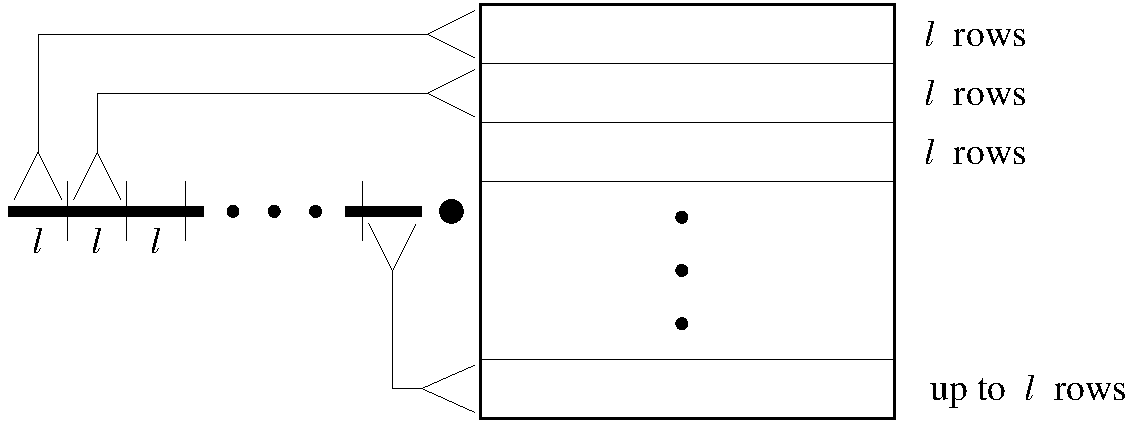
\includegraphics[width=13cm]{grease}
\end{center}
\caption{Illustration for Vector-matrix multiplication and grease}
\label{grease}
\end{figure}

\subsection{Matrix multiplication}

Greasing.

\subsection{Matrix inversion}

Greasing.

\subsection{Semi echelonisation}

Cleaning, spinning.

\section{Cache issues}
\label{sec:cache}

Expected performance gain, problems.

\section{Characteristic and minimal polynomial}
\label{sec:charminpoly}

\section{Basic algorithms for matrices}
\label{sec:basalgmat}

Evaluation of polynomials at matrices, order of an invertible matrix.

